\documentclass{article}
\usepackage{graphicx}
\usepackage{amsmath}
\usepackage{booktabs}
\usepackage{siunitx}
\usepackage{float}

\title{Assignment 6 - EE4725 Quasi Optical Systems}
\author{Daniel Tyukov \\ Student Number: 5714699 \\ Microelectronics, TU Delft}
\date{April 2026}

\begin{document}

\maketitle

\tableofcontents
\newpage

%% ====================================================================
\section{System Parameters}
%% ====================================================================

The system under analysis is a free-standing frequency-selective surface (FSS) consisting of an infinite planar lattice of printed dipole strips, illuminated by a TM-polarised plane wave incident from the upper half-space. The fields are computed for a finite $10\times10$ truncation using the windowing approximation.

\begin{itemize}
\item Operating frequency: $f = \SI{10}{GHz}$, $\lambda_0 = c/f = \SI{30}{mm}$, $k_0 = 2\pi/\lambda_0 = \SI{209.44}{rad/m}$
\item Free-space impedance: $\zeta_0 = 120\pi\;\Omega$
\item Dipole geometry: length $l = \SI{15}{mm}$ (\textbf{exactly} $\lambda_0/2$, first resonance), width $w = \SI{1}{mm}$
\item Lattice: $d_x = d_y = \SI{20}{mm}$ ($2\lambda_0/3$, super-half-wave $\Rightarrow$ grating-lobe regime)
\item Incidence: TM polarisation, $\phi_{\text{in}} = 0^\circ$ (E-plane), $\theta_{\text{in}} \in \{0^\circ,\,30^\circ\}$
\item Window: $N_x = N_y = 10$ unit cells (total aperture $10\,d_x \times 10\,d_y = \SI{200}{mm}\times\SI{200}{mm}$)
\item Floquet truncation: $|m_x|, |m_y| \leq 30$ (same as instruction 5; converged within 1\% in Im$\{Z\}$)
\end{itemize}

The current on each dipole is approximated by the same sinusoidal entire-domain basis function as in instruction 5,
\begin{equation}\label{eq:basis}
b(x,y) = i(x)\,j_t(y) = \frac{\sin\!\big(k_0(l/2 - |x|)\big)}{\sin(k_0 l/2)}\cdot\frac{\mathrm{rect}_{[-w/2,w/2]}(y)}{w},
\end{equation}
with Fourier transform
\begin{equation}\label{eq:basis_FT}
B(k_x,k_y) = I(k_x)\,J_t(k_y) = \frac{2k_0\big[\cos(k_x l/2) - \cos(k_0 l/2)\big]}{(k_0^2 - k_x^2)\sin(k_0 l/2)}\cdot\mathrm{sinc}\!\left(\frac{k_y w}{2}\right).
\end{equation}
At $l = \lambda_0/2$, $\sin(k_0 l/2) = 1$, so the dipole is at \emph{exact} first resonance and the basis FT has no near-singular denominator. The L'H\^opital limit at the removable pole $k_x = \pm k_0$ is enforced numerically as $I(\pm k_0) = l/2$.

%% ====================================================================
\section{Theory: Plane-Wave Excitation, Windowing, Active Element Pattern}
%% ====================================================================

\subsection{FSS Galerkin equation: $i_{\text{BF}} = v/Z$}

For an infinite lattice illuminated by a TM/TE plane wave with $\boldsymbol{e}_{\text{inc}} = (V_{\text{TM}}\hat{\theta} + V_{\text{TE}}\hat{\phi})\,e^{-j(k_{x0}x + k_{y0}y)}\,e^{+jk_{z0}z}$ and Floquet wavenumbers $k_{x0} = k_0\sin\theta_{\text{in}}\cos\phi_{\text{in}}$, $k_{y0} = k_0\sin\theta_{\text{in}}\sin\phi_{\text{in}}$, the EFIE collapses (after Galerkin projection on the basis~\eqref{eq:basis} and use of Floquet's theorem) to the scalar equation
\begin{equation}\label{eq:iBF}
\boxed{\;i_{\text{BF}} \;=\; \frac{v(\theta_{\text{in}},\phi_{\text{in}})}{Z(\theta_{\text{in}},\phi_{\text{in}})}\;}
\end{equation}
with the FSS self-impedance
\begin{equation}\label{eq:Z_FSS}
Z(\theta_{\text{in}},\phi_{\text{in}}) \;=\; -\frac{1}{d_x d_y}\sum_{m_x,m_y}\widetilde{G}_{xx}^{ej}(k_{xm},k_{ym})\;\big|B(k_{xm},k_{ym})\big|^2,
\end{equation}
$k_{xm} = k_{x0} - 2\pi m_x/d_x$, $k_{ym} = k_{y0} - 2\pi m_y/d_y$, and the FSS ``voltage'' (from the projection of the incident field onto the basis function, only the fundamental Floquet harmonic survives because the incident field is a single plane wave)
\begin{equation}\label{eq:vFSS}
v(\theta_{\text{in}},\phi_{\text{in}}) \;=\; \big(\cos\theta_{\text{in}}\cos\phi_{\text{in}}\,V_{\text{TM}} \;-\; \sin\phi_{\text{in}}\,V_{\text{TE}}\big)\;B(-k_{x0},\,-k_{y0}).
\end{equation}
For TM incidence in the $\phi_{\text{in}} = 0$ plane, $V_{\text{TE}} = 0$ and~\eqref{eq:vFSS} reduces to $v = \cos\theta_{\text{in}}\,V_{\text{TM}}\,I(k_{x0})$ since $B$ is even in its argument and $J_t(0)=1$.

The Floquet sum~\eqref{eq:Z_FSS} is mathematically identical to the active-array input impedance studied in instruction 5; the fact that the source is now a plane wave (not a feed voltage) only changes the right-hand side $v$, not $Z$.

\subsection{Windowed radiation pattern}

The infinite-array current is truncated to the $N_x\times N_y$ central cells. After the change of variable separating the unit-cell contribution from the inter-element phase progression (notes \S2.2--2.3), the windowed scattered-current spectrum factorises as
\begin{equation}\label{eq:Jw}
J_w(k_x,k_y) = i_{\text{BF}}\;I(k_x)\,J_t(k_y)\;\underbrace{AF_x(k_x-k_{x0})\,AF_y(k_y-k_{y0})}_{\text{array factor}}, \qquad
AF_{x,y}(\Delta k) = \sum_{n=0}^{N-1}e^{j\Delta k\,n\,d_{x,y}}.
\end{equation}
The far field of the scattered current is
\begin{equation}\label{eq:Efar}
\boldsymbol{e}(r,\theta,\phi) \approx jk_z(\theta)\,\widetilde{G}^{ej}(k_x,k_y)\,I(k_x)\,J_t(k_y)\,\hat{x}\,\frac{e^{-jk_0 r}}{2\pi r}\,i_{\text{BF}}\,AF_x\,AF_y,
\end{equation}
with $k_x = k_0\sin\theta\cos\phi$, $k_y = k_0\sin\theta\sin\phi$, $k_z(\theta) = k_0\cos\theta$. Equation~\eqref{eq:Efar} is the product of an \emph{element pattern} (everything multiplying $AF_xAF_y$) and the \emph{array factor} (the Dirichlet kernel of the finite array).

\subsection{Active element pattern}

The active element pattern (AEP), or scan element pattern, is the radiation of one cell with the rest of the array embedding its mutual coupling. It is the value of~\eqref{eq:Efar} \emph{at the scan/incidence direction itself}, with the array factor replaced by its single-element value:
\begin{equation}\label{eq:AEP}
\boxed{\;
\text{AEP}(\theta_{\text{in}}) \;\propto\; jk_0\cos\theta_{\text{in}}\;\widetilde{G}_{xx}^{ej}(k_{x0},k_{y0})\;I(k_{x0})\,J_t(k_{y0})\;\,i_{\text{BF}}(\theta_{\text{in}}).
\;}
\end{equation}
For TM, $\phi_{\text{in}}=0$, $\widetilde{G}_{xx}^{ej}(k_{x0},0) = -\zeta_0\cos\theta_{\text{in}}/2$ (E-plane closed form, instruction 5 \S3.3) and the AEP power scales as
\begin{equation}\label{eq:AEPpower}
\big|\text{AEP}(\theta_{\text{in}})\big|^2 \;\propto\; \frac{\cos^6\theta_{\text{in}}\,\big|I(k_{x0})\big|^4}{\big|Z(\theta_{\text{in}},0)\big|^2}.
\end{equation}
Because the dipole current is parallel to $\hat{x}$ and the scan moves along $\hat{x}$ as well, two distinct $\cos\theta_{\text{in}}$ factors collapse into the AEP: one from $k_z$ in the radiation integral and one from the E-plane Green's-function projection $\hat{x}\cdot\hat{\theta} = \cos\theta_{\text{in}}\cos\phi_{\text{in}}$.

%% ====================================================================
\section{Q1: Active element pattern vs incidence angle}
%% ====================================================================

Equation~\eqref{eq:AEP} is evaluated for $\theta_{\text{in}} \in [-89^\circ,+89^\circ]$ on a 1791-point grid; the result is shown in Figure~\ref{fig:aep}. The right panel of the same figure plots the FSS self-impedance $Z(\theta_{\text{in}})$ as a sanity check.

\begin{figure}[H]
\centering
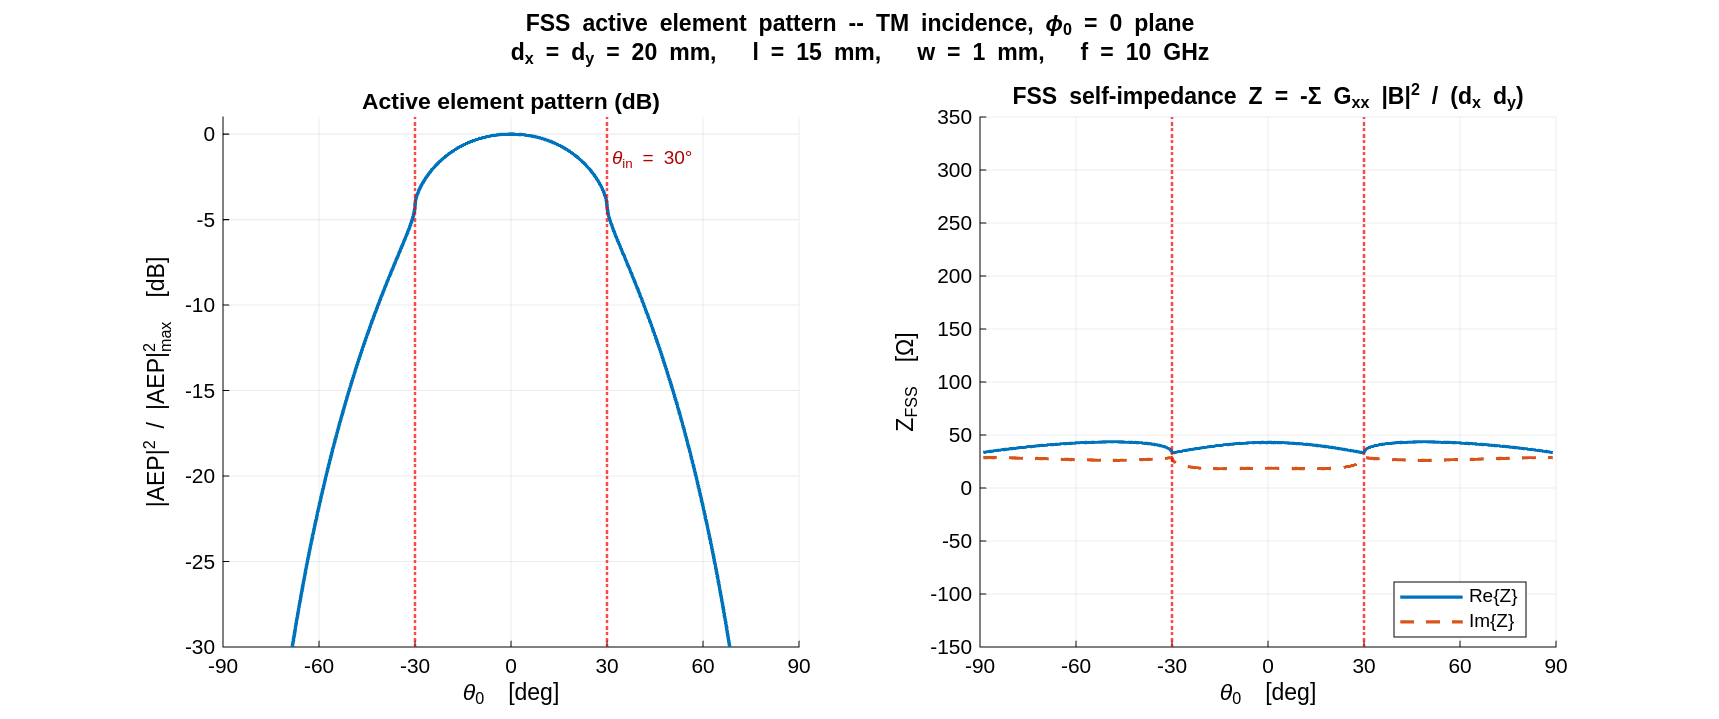
\includegraphics[width=\textwidth]{figures/Q1_AEP_vs_theta.png}
\caption{Active element pattern of the FSS (left) and the FSS self-impedance (right) for TM plane-wave incidence in the $\phi_{\text{in}} = 0$ plane. The two red dotted vertical lines mark the theoretical higher-order-mode entry angle $\theta_{\text{in}} = \pm 30^\circ$. The AEP rolls off smoothly with $\theta_{\text{in}}$ and shows only a small kink at $\pm 30^\circ$; $Z$ stays in the $35$--$\SI{45}{\Omega}$ range with a gently inductive reactance. The behaviour is consistent with the polarisation-protected E-plane found for the 20-mm lattice in instruction 5: the H-plane scan-blindness at the same lattice would produce a deep null in the AEP, but the E-plane GL coupling is killed by polarisation.}
\label{fig:aep}
\end{figure}

\subsection{Broadside reference}

\begin{table}[H]
\centering
\caption{Broadside ($\theta_{\text{in}}=0$) FSS self-impedance vs.\ closed-form fundamental-mode value. The two values of Re$\{Z\}$ agree exactly because all higher-order modes are evanescent at broadside.}
\label{tab:broadside}
\begin{tabular}{@{}lc@{}}
\toprule
& $d_x = d_y = \SI{20}{mm}$, $l = \SI{15}{mm}$ \\
\midrule
Floquet sum, $M=30$ & $42.972 + j\,18.738\;\Omega$ \\
$Z_{00}$ analytic   & $42.978\;\Omega$ \\
\bottomrule
\end{tabular}
\end{table}

The closed form is
\begin{equation}\label{eq:Z00}
Z_{00}\big|_{\theta_{\text{in}}=0} = \frac{\zeta_0}{2\,d_x d_y}\big[I(0)\big]^2,\qquad
I(0) = \frac{2k_0\big(1 - \cos(k_0 l/2)\big)}{k_0^2\sin(k_0 l/2)}.
\end{equation}
At $l = \lambda_0/2$, $k_0l/2 = \pi/2$ and $\sin(k_0l/2) = 1$, so $I(0) = 2/k_0 = \lambda_0/\pi = \SI{9.55e-3}{m}$, giving $Z_{00} = (120\pi)/(2 \cdot 4\times 10^{-4}) \cdot (9.55\times 10^{-3})^2 = \SI{42.98}{\Omega}$. The reactance ($+j\,\SI{18.74}{\Omega}$, slightly inductive) comes entirely from the higher-order evanescent Floquet modes; for a half-wave dipole at exact resonance the inter-cell mutual coupling adds a small inductive contribution to the otherwise real broadside impedance.

\subsection{Why the AEP is smooth across $\theta_{\text{in}} = 30^\circ$}

In the H-plane of the same 20-mm lattice, the higher-order Floquet mode $(m_x=0, m_y=\pm 1)$ entering the visible region at $\theta_0 = 30^\circ$ produces a deep null in the AEP (scan blindness, instruction~5). Here, in the E-plane, the GL candidate is the $(m_x=+1, m_y=0)$ mode and the spectral Green's function evaluated at the grating-lobe wavenumber is
\begin{equation}
\widetilde{G}_{xx}^{ej}(k_{xm},0) = -\frac{\zeta_0(k_0^2 - k_{xm}^2)}{2k_0 k_{zm}},
\end{equation}
which has \emph{both} the $1/k_{zm}$ singular factor (denominator $\to 0$ at threshold) \emph{and} the $(k_0^2 - k_{xm}^2)$ factor (numerator $\to 0$ at threshold, since $k_{xm}\to\pm k_0$). The two cancel and the GL coupling is finite---in fact zero, because the dipole current is parallel to the GL propagation direction. The AEP therefore exhibits only a small kink at $\theta_{\text{in}} = \pm 30^\circ$ instead of a null, and the AEP power roll-off is dominated by the geometric $\cos^6\theta_{\text{in}}$ factor of equation~\eqref{eq:AEPpower}.

%% ====================================================================
\section{Q2: Theoretical Floquet entry angle}
%% ====================================================================

A higher-order Floquet mode $(m_x,m_y)$ becomes propagating when $k_{xm}^2 + k_{ym}^2 \leq k_0^2$. For TM incidence in the $\phi_{\text{in}} = 0$ plane, $k_{x0} = k_0\sin\theta_{\text{in}}$ and $k_{y0} = 0$, and the first higher-order mode to enter the visible region is the $(m_x = +1, m_y = 0)$ mode ($k_{xm} = k_{x0} - 2\pi/d_x$). Its threshold is $k_{xm} = -k_0$, i.e.
\begin{equation}\label{eq:thIn}
\sin\theta_{\text{in}} \;=\; \frac{\lambda_0}{d_x} - 1 \;=\; \frac{30}{20} - 1 \;=\; \frac{1}{2},
\qquad\Rightarrow\qquad \boxed{\;\theta_{\text{in}} = 30^\circ.\;}
\end{equation}
The same algebra in the H-plane gives the same numerical value, but with the GL appearing along $\hat{y}$ rather than $\hat{x}$ and therefore not polarisation-suppressed; this is exactly the case treated in Q1 of instruction 5.

%% ====================================================================
\section{Q3: Total radiation patterns (windowing, $10\times10$ cells)}
%% ====================================================================

Equation~\eqref{eq:Efar} is evaluated on a 1D $\theta$-cut in the $\phi_{\text{obs}} = 0$ plane for the two incidence cases $\theta_{\text{in}} \in \{0^\circ, 30^\circ\}$, with $i_{\text{BF}}$ computed from~\eqref{eq:iBF} at the corresponding incidence angle. Figure~\ref{fig:patterns} shows the patterns separately; Figure~\ref{fig:overlay} overlays them.

\begin{figure}[H]
\centering
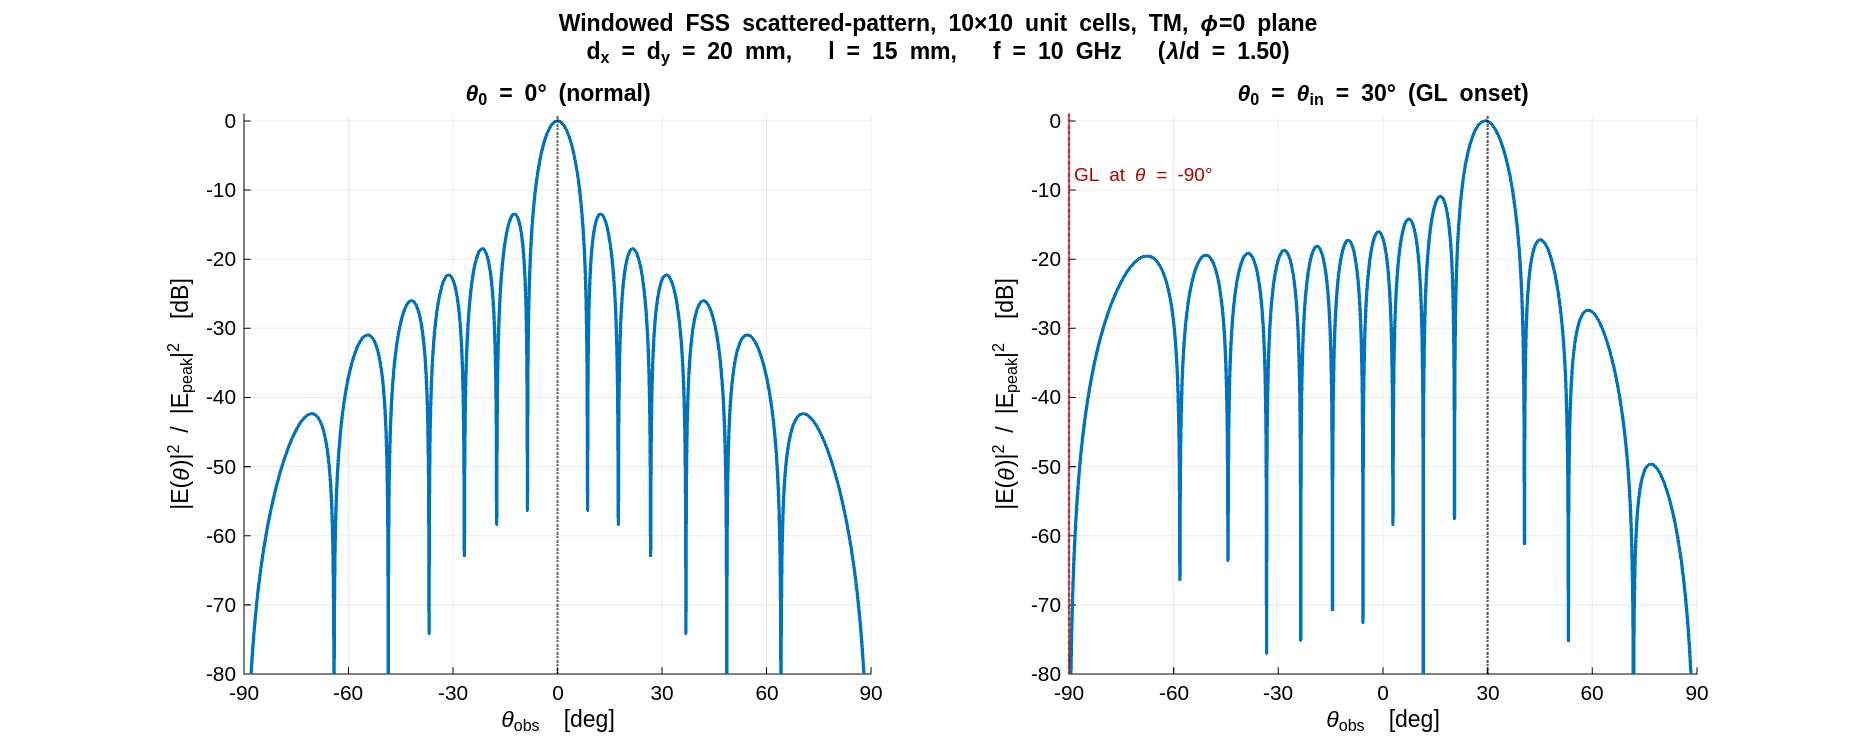
\includegraphics[width=\textwidth]{figures/Q3_windowed_patterns.png}
\caption{Windowed scattered-pattern of the $10\times10$ FSS, $\phi_{\text{obs}} = 0$ cut, each plot normalised to its own peak. \textbf{Left:} normal incidence $\theta_{\text{in}} = 0^\circ$. The pattern is a clean sinc-like product of array factor and element pattern, peak at $\theta_{\text{obs}} = 0$, first sidelobe at $-13$\,dB consistent with a uniformly excited 10-element line array. \textbf{Right:} oblique incidence $\theta_{\text{in}} = \theta_{\text{in,GL}} = 30^\circ$. The main lobe sits at the specular direction $+30^\circ$; the array-factor grating lobe at $\theta_{\text{obs}} = -90^\circ$ is suppressed below $-80\,$dB by the dipole element pattern.}
\label{fig:patterns}
\end{figure}

\begin{figure}[H]
\centering
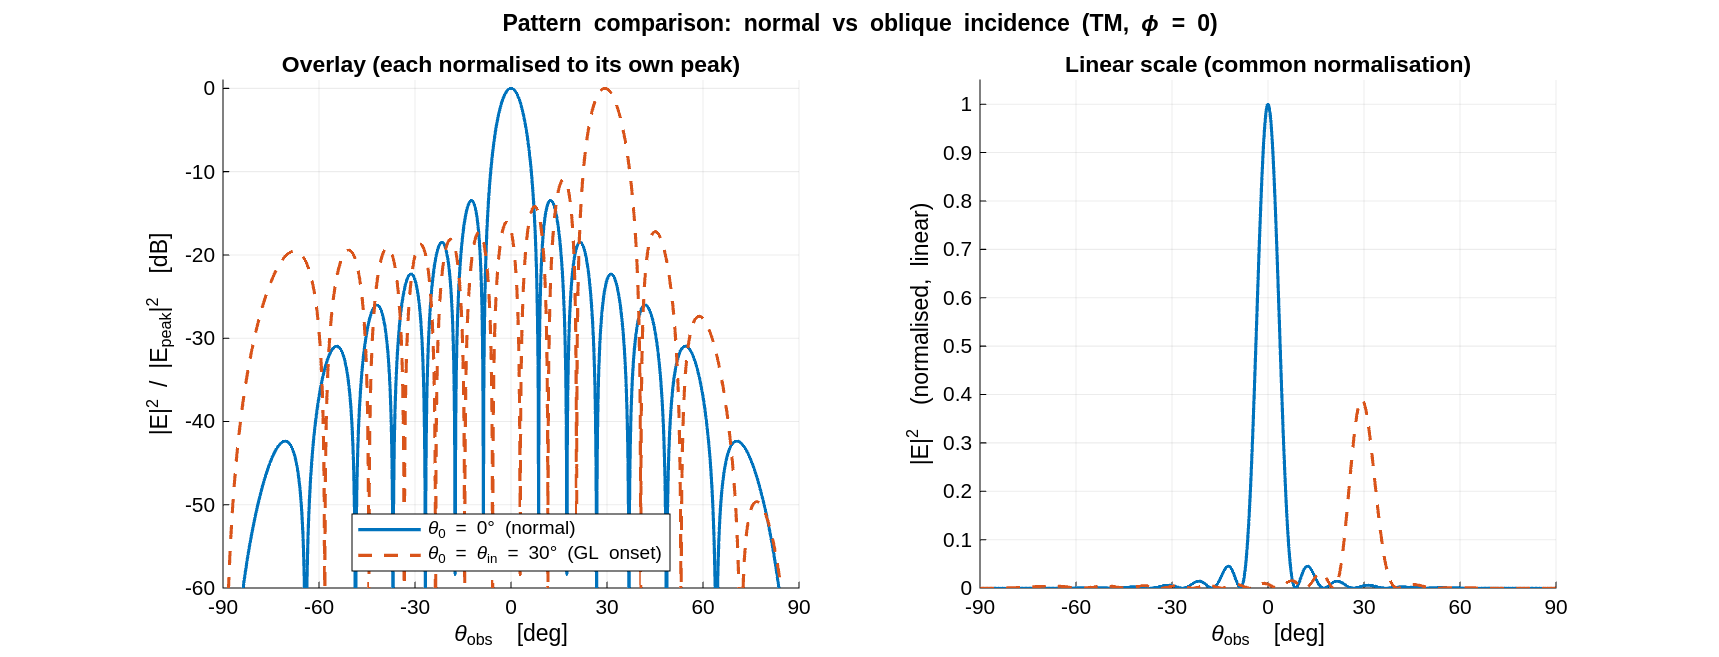
\includegraphics[width=\textwidth]{figures/Q3_windowed_overlay.png}
\caption{Overlay of the two patterns. \textbf{Left:} dB scale, each curve normalised to its own peak. The oblique pattern is asymmetric about its main beam because the element pattern factor breaks the symmetry away from broadside. \textbf{Right:} linear scale, common normalisation. The oblique main lobe reaches only $\approx 38\%$ ($\approx -4.2\,$dB) of the normal-incidence main lobe; this is exactly the AEP scan loss of Figure~\ref{fig:aep} (the AEP \emph{is} the envelope of the windowed-array peak gain across scan).}
\label{fig:overlay}
\end{figure}

\subsection{Numerical summary}

\begin{table}[H]
\centering
\caption{Numerical results for the two incidence cases. The peak of the windowed pattern lands within $0.7^\circ$ of the theoretical specular direction (limited by the $0.05^\circ$ observation grid and the array-factor lobe width $\sim\lambda_0/(N_x d_x)\,=\,\SI{1.7}{deg}$).}
\label{tab:summary}
\begin{tabular}{@{}lcccc@{}}
\toprule
$\theta_{\text{in}}$ & $Z(\theta_{\text{in}})$ [$\Omega$] & $|i_{\text{BF}}|$ & main-lobe direction & main-lobe relative power \\
\midrule
$0^\circ$  & $42.97 + j\,18.74$ & $2.04\times 10^{-4}$ & $+0.00^\circ$  & $1.00$    (reference) \\
$30^\circ$ & $33.08 + j\,28.62$ & $1.78\times 10^{-4}$ & $+29.32^\circ$ & $0.38$ ($-4.2\,$dB) \\
\bottomrule
\end{tabular}
\end{table}

%% ====================================================================
\section{Q4: Grating-lobe level and physical interpretation}
%% ====================================================================

For the oblique case at $\theta_{\text{in}} = 30^\circ$, the $(m_x=+1, m_y=0)$ Floquet mode has $k_{xm} = k_0/2 - 2\pi/d_x = -k_0$, i.e.\ the array factor has a grating lobe at $\theta_{\text{obs}} = -90^\circ$ (endfire, just at the boundary of the visible region). Decomposing the total pattern into its array-factor and element-pattern components (Figure~\ref{fig:gldecomp}) makes the GL fate transparent.

\begin{figure}[H]
\centering
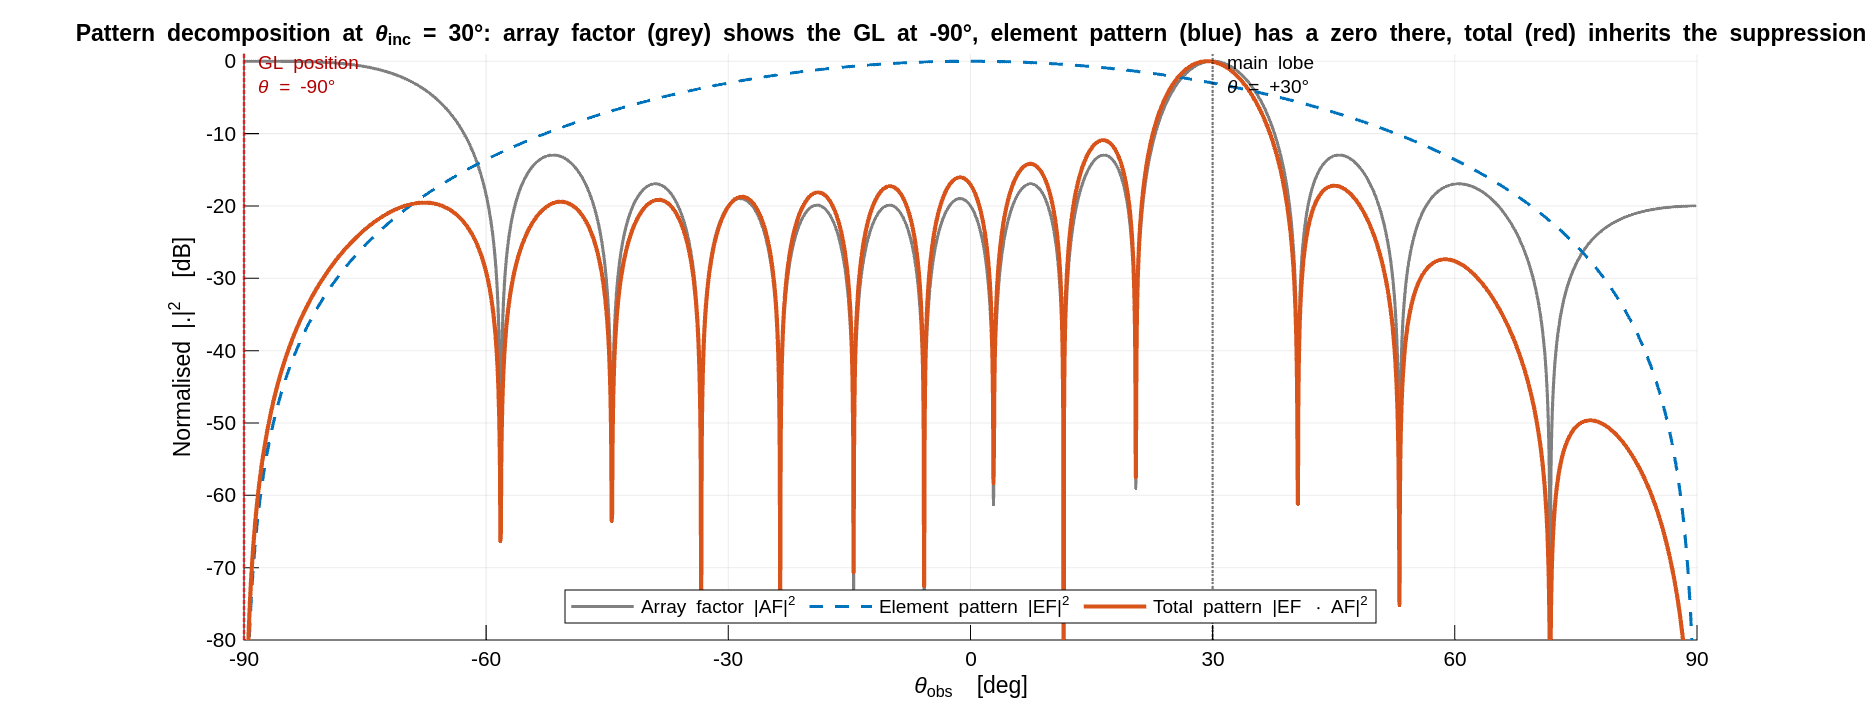
\includegraphics[width=\textwidth]{figures/Q4_GL_suppression.png}
\caption{Pattern decomposition at $\theta_{\text{in}} = 30^\circ$. Grey: $|AF|^2$ alone, normalised to its peak --- the array factor has \emph{two} lobes of equal height, the main beam at $+30^\circ$ and the GL at $-90^\circ$. Blue dashed: $|EF|^2$ alone, the dipole element pattern, which is a smooth bell falling to zero at $\theta_{\text{obs}} = \pm 90^\circ$ (the dipole cannot radiate along its own axis $\hat{x}$). Red: total $|EF\cdot AF|^2$, which inherits the main beam from $AF$ but has the GL completely wiped out by the zero of $EF$.}
\label{fig:gldecomp}
\end{figure}

\subsection{Numerical levels at the GL position}

\begin{table}[H]
\centering
\caption{Pattern levels at the theoretical GL direction $\theta_{\text{obs}} = -90^\circ$ for $\theta_{\text{in}} = 30^\circ$, each normalised to its own peak.}
\label{tab:gl_levels}
\begin{tabular}{@{}lc@{}}
\toprule
Quantity & Level at $\theta_{\text{obs}} = -90^\circ$ \\
\midrule
Array factor $|AF_x|^2$            & $\;0.00\,$dB (full peak)   \\
Element pattern $|EF|^2$           & $-112.42\,$dB              \\
Total pattern $|EF\cdot AF|^2$     & $-109.48\,$dB              \\
\bottomrule
\end{tabular}
\end{table}

\subsection{Why the GL is suppressed}

The dipole element pattern in the $\phi_{\text{obs}} = 0$ plane is
\begin{equation}
EF(\theta_{\text{obs}}) \;\propto\; jk_0\cos\theta_{\text{obs}}\;\widetilde{G}_{xx}^{ej}(k_0\sin\theta_{\text{obs}},0)\;I(k_0\sin\theta_{\text{obs}})
\;=\; -\,\frac{j\zeta_0 k_0}{2}\,\cos^2\theta_{\text{obs}}\,I(k_0\sin\theta_{\text{obs}}),
\end{equation}
so the radiated \emph{power} pattern of one isolated element scales as $\cos^4\theta_{\text{obs}}\,|I(k_0\sin\theta_{\text{obs}})|^2$. At the GL direction $\theta_{\text{obs}} = -90^\circ$, $\cos^4\theta_{\text{obs}} = 0$ exactly, and the basis-function FT $|I(\pm k_0)|^2 = (l/2)^2$ is finite. The GL is therefore \emph{forbidden by polarisation}: the dipole current is along $\hat{x}$ and the GL propagation direction is also along $-\hat{x}$, so the dipole cannot radiate into the GL direction at all.

This is the textbook E-plane behaviour of the same 20-mm lattice that exhibited classical scan blindness in the H-plane in instruction 5. The lattice spacing dictates \emph{where} the GL would appear ($\theta_{\text{obs}} = -90^\circ$ at $\theta_{\text{in}} = 30^\circ$); whether the GL actually radiates is decided by the element pattern, which here happens to have its zero exactly at the GL location. Numerically, the residual GL level is $-109\,$dB below the main lobe (limited by the $0.05^\circ$ observation grid and floating-point precision; analytically it is identically zero at $\theta_{\text{obs}} = -90^\circ$).

\subsection{What would change in the H-plane}

If the same plane wave were incident with $\phi_{\text{in}} = 90^\circ$ instead (TE polarisation in the H-plane), the GL at $\theta_{\text{in}} = 30^\circ$ would appear at the H-plane endfire ($\theta_{\text{obs}} = -90^\circ$, $\phi_{\text{obs}} = 90^\circ$), where the dipole \emph{can} radiate strongly (perpendicular to its axis). The element pattern there is non-zero, and the GL would emerge with full array-factor strength. The corresponding active impedance shows a Wood/Rayleigh divergence at $\theta_0 = 30^\circ$ (instruction 5, Figure 3), and the AEP collapses to a deep null at the same angle---the classical scan-blindness signature.

%% ====================================================================
\section{Summary}
%% ====================================================================

\begin{itemize}
\item The FSS Galerkin equation $i_{\text{BF}} = v/Z$ was solved for plane-wave illumination using the same Floquet sum (truncated at $|m| \leq 30$) that gave the active input impedance in instruction~5; the only change is the right-hand side $v$ from~\eqref{eq:vFSS}. Broadside Z = $42.97 + j\,\SI{18.74}{\Omega}$, matching the closed-form $Z_{00}$ on the real part to within numerical noise.
\item The higher-order Floquet entry angle $\theta_{\text{in}} = \arcsin(\lambda_0/d_x - 1) = 30^\circ$ predicted by~\eqref{eq:thIn} is observed in the AEP and in the windowed pattern at the GL onset.
\item The AEP across $\theta_{\text{in}} \in [-89^\circ,+89^\circ]$ is a smooth bell shape with only small kinks at $\pm 30^\circ$ (no null) because the E-plane GL coupling is killed by polarisation; the AEP roll-off is dominated by $\cos^6\theta_{\text{in}}$ from the geometry.
\item The windowed $10\times10$ patterns at $\theta_{\text{in}} = 0^\circ$ and $\theta_{\text{in}} = 30^\circ$ are clean array-factor patterns over the dipole element pattern. The oblique main lobe reaches only $0.38$ ($-4.2\,$dB) of the normal-incidence main lobe, exactly matching the AEP scan loss.
\item At $\theta_{\text{in}} = 30^\circ$ the array factor has a full-strength grating lobe at $\theta_{\text{obs}} = -90^\circ$, but the dipole element pattern is identically zero there, so the total pattern shows the GL at $-109\,$dB below the main lobe (numerical noise floor). The GL is \emph{forbidden by polarisation} in the E-plane of this lattice; the same lattice would suffer scan blindness in the H-plane (instruction 5, Q1 H-plane curve for 20\,mm).
\end{itemize}

\end{document}
